\documentclass[a4paper, 12pt]{article}
\usepackage[T1]{fontenc}
\usepackage{lmodern}
\usepackage{color}
\usepackage{amsfonts}
\usepackage{epstopdf}
\usepackage{matlab}
\usepackage{booktabs}
%\documentclass{book}
\usepackage{blindtext}
\usepackage{hyperref}
\usepackage[brazil]{babel}
\usepackage{amssymb}
\usepackage[utf8]{inputenc}
\usepackage{amsmath}
\usepackage{indentfirst}
\usepackage{graphicx}
\usepackage{listings}
\usepackage{tcolorbox}
\usepackage{upgreek}
\usepackage{multicol,lipsum}
\usepackage[a4paper,
top=3cm, left=3cm, bottom=3cm, right=3cm]{geometry}
\usepackage{setspace}
\usepackage{multirow}
\usepackage{float}
\usepackage[dvipsnames]{xcolor}
\usepackage[table]{xcolor}
%\usepackage{pdflscape}
\usepackage[DIV=15]{typearea}
\usepackage[nottoc]{tocbibind}
\usepackage[sort,numbers]{natbib}
%\usepackage{cite}
\usepackage{matlab}

\usepackage[utf8]{inputenc}
\usepackage[T1]{fontenc}
\usepackage{lmodern}
\usepackage{graphicx}
\usepackage{color}
\usepackage{hyperref}
\usepackage{amsmath}
\usepackage{amsfonts}
\usepackage{epstopdf}
\usepackage[table]{xcolor}
\usepackage{matlab}

\lstdefinestyle{python}{
  language=Python,
  basicstyle=\ttfamily,
  keywordstyle=\color{blue},
  stringstyle=\color{green},
  commentstyle=\color{gray},
  numbers=left,
  numberstyle=\tiny\color{gray},
  stepnumber=1,
  numbersep=5pt,
  backgroundcolor=\color{white},
  showspaces=false,
  showstringspaces=false,
  showtabs=false,
  frame=single,
  rulecolor=\color{black},
  tabsize=4,
  captionpos=b,
  breaklines=true,
  breakatwhitespace=false,
  title=\lstname,
  escapeinside={\%*}{*)},
  morekeywords={self},
  emph={MyClass,__init__},
  emphstyle=\color{red}
}


\documentclass[letterpaper]{article}
% bib pack %%%%%%%%%%%%%%%%%%%%%%%%%%%%%%%%%%%%%%%%%%%%%%%%%%%%%%%%%%%%%%%%%%%%%
\usepackage[utf8]{inputenc}
\usepackage{geometry}
    \geometry{left=3cm,right=2cm,top=2cm,bottom=2cm}
%
\usepackage[spanish]{babel}
%
\usepackage[fixlanguage]{babelbib}
    \bibliographystyle{babunsrt}
%
\usepackage{url}

\begin{document}
%\maketitle

\begin{titlepage}
	\begin{center}
		

\vspace{10pt}
%\begin{figure}[H][!ht]
%\centering
%
\includegraphics{puc-rio-logo.png}

%\end{figure}
\begin{figure}[!ht]
\centering

\includegraphics{images/puc-rio-logo.png}
\end{figure}
\huge{Inteligência Computacional Aplicada}
        \vspace{70pt}
        
		\textbf{ENG1456}
		\textbf{\large{\\ }}
		
		\vspace{30pt}
		\textbf{\small{\\TRABALHO 1}}
            \textbf{\small{\\Algoritmos Genéticos}}
		\vspace{75pt}
		
	\end{center}
	
	\begin{flushleft}
		\begin{tabbing}
		Aluno(a)\qquad\qquad\=\>Paloma Fernanda Loureiro Sette - 1621595\\
  Aluno(a)\qquad\qquad\=\>Renata Boeck Miranda - 2110702\\
			Professor(a)\>Karla Figueiredo\\
	\end{tabbing}
		  
	\end{flushleft}
	\begin{center}
		%\vspace{\fill}
		\vspace{215pt}
		Rio de Janeiro, 12 de Maio de 2024
	\end{center}
\end{titlepage}
%%%%%%%%%%%%%%%%%%%%%%%%%%%%%%%%%%%%%%%%%%%%%%%%%%%%%%%%%%%
\newpage
\tableofcontents
\thispagestyle{empty}

\newpage
\pagenumbering{arabic}

\newpage

%\newcommand{\listequationsname}{Lista de Equações}
%\newlistof{myequations}{equ}{\listequationsname}
%\newcommand{\myequations}[1]{%
%\addcontentsline{equ}{myequations}{\protect\numberline{\theequation}#1}\par}

%\listofmyequations
\newpage


\newpage

\listoffigures
\thispagestyle{empty}

\newpage
%%%%%%%%%%%%%%%%%%%%%%%%%%%%%%%%%%%%%%%%%%%%%%%%%%%%%%%%%
%%%%%%%%%%%%%%%%%%%%%%%%%%%%%%%%%%%%%%%%%%%%%%%%%%%

\newpage

\thispagestyle{empty}

\newpage

\section*{Introdução}
Este relatório refere-se ao primeiro trabalho de algoritmos genéticos da disciplina de Inteligência Computacional Aplicada (2024.1), cujo problema a ser otimizado é a Função Binária $f_6$.\\

Utilizaremos o software GAdemo e o crossover de 1 (um) ponto para os experimentos.

\begin{figure}[H]
\centering
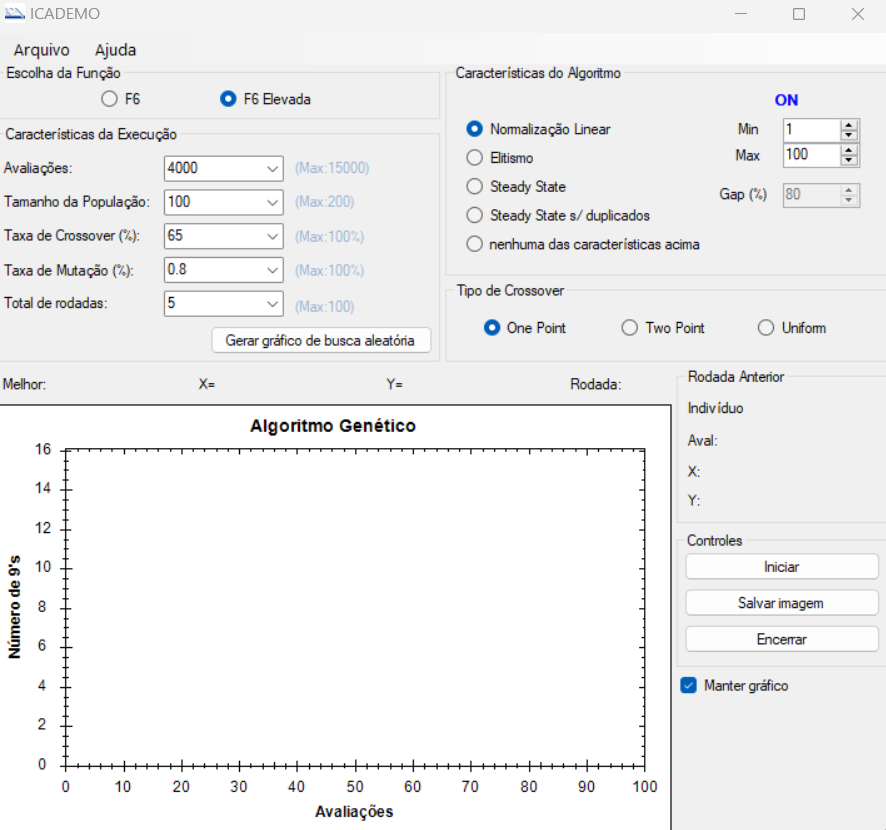
\includegraphics[scale = 0.70]{images/gademo.PNG}
\caption{Interface do GAdemo}
\end{figure}


\newpage
\section{Taxas de Crossover e Mutação}
\textbf{Variando os parâmetros, devemos executar Algoritmos Genéticos cujos parâmetros são apresentados na tabela abaixo. O intuito é comparar e explicar os resultados 
obtidos com as curvas referentes à média de 20 rodadas de cada GA.}\\

Incluir dois gráficos: um com GA1-1, GA2-1 e GA2-2 e outro com GA2-3 e GA2-4.

\begin{figure}[H]
\centering
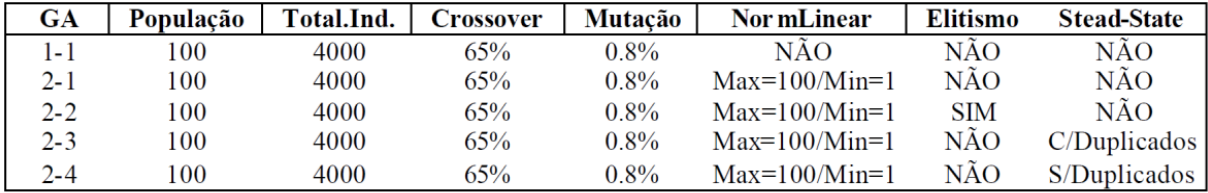
\includegraphics[scale = 0.55]{images/table_1.png}
\end{figure}

\subsection{GA1-1, GA2-1 e GA2-2}

\begin{figure}[H]
\centering
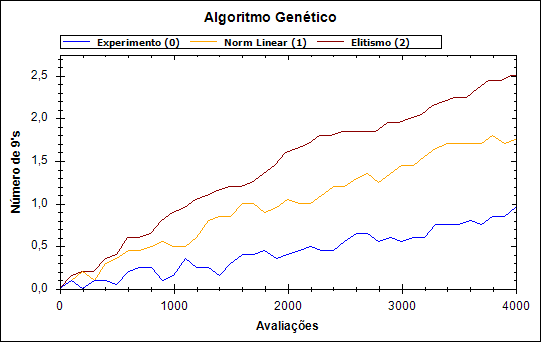
\includegraphics[scale = 0.95]{images/q1.1.png}
\caption{GA1-1, GA2-1 e GA2-2}
\end{figure}

\textbf{GA1-1 (Azul)}: Sem ajustes de normalização linear ou steady state, mostra uma progressão constante e uma melhora relativamente estável ao longo das avaliações.\\

\textbf{GA2-1 (Laranja)}: Com normalização linear em uma configuração ligeiramente diferente (ainda assim, parece seguir a mesma linha de base que GA1-1, indicando que as mudanças entre GA1 e GA2 podem não ser tão significativas nesta configuração específica).\\

\textbf{GA2-2 (Marrom)}: Com normalização linear e elitismo, mostra uma melhora significativa em relação aos outros dois. A normalização linear juntamente com elitismo parece ajudar na eficiência do algoritmo em encontrar melhores soluções mais rapidamente.\\



\subsection{GA2-3 e GA2-4}

\begin{figure}[H]
\centering
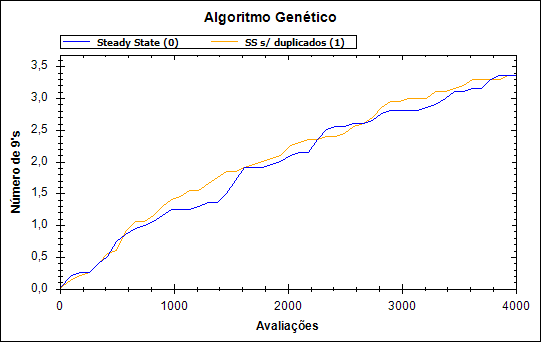
\includegraphics[scale = 0.95]{images/q1.2.png}
\caption{GA2-3 e GA2-4}
\end{figure}

\textbf{GA2-3 (Azul)}: Utilizando steady state com duplicados, percebemos um aumento gradual e consistente, sugerindo que a manutenção de uma diversidade com duplicatas pode estar contribuindo para uma exploração eficaz do espaço de busca.\\

\textbf{GA2-4 (Laranja)}: Com steady state e sem duplicados, este também mostra uma tendência de melhoria contínua, mas com uma performance levemente superior à do GA2-3. A eliminação de duplicatas parece ter um impacto positivo, possibilitando que o algoritmo evite convergências prematuras e explore mais profundamente o espaço de soluções.\\

\subsection{Conclusões}

Os resultados indicam que a normalização linear (GA2-2) pode ser muito útil para melhorar a performance dos algoritmos em problemas onde a diversidade de soluções e a prevenção de convergências prematuras são cruciais.\\

Os algoritmos que utilizam steady state, especialmente quando combinados com a prevenção de duplicatas (GA2-4), mostram uma melhoria significativa em sustentar o progresso ao longo das gerações, sugerindo que essa técnica é benéfica para manter a diversidade genética e explorar eficientemente o espaço de busca.



%%%%%%%%%%%%%%%%%%%%%%%%%%%%%%%%%%%%%
\newpage
\section{Algoritmos Genéticos que utilizam Steady-State}
\textbf{Para os GAs que utilizam steady-state, devemos determinar o GAP (número de indivíduos substituídos a cada ciclo) 
ideal. Para isso, deveremos usar um incremento de 5 indivíduos a cada tentativa, começando com um GAP=5.} \\

Foram realizadas 12 tentativas, resultando em um total de 60 GAPs. As imagens seguintes demonstram o gráfico resultante. O conjunto de gráficos expande as observações sobre como diferentes valores de GAP influenciam a performance do algoritmo genético no modelo Steady State. A visualização inclui uma gama ampla de GAPs, permitindo uma comparação detalhada.

\begin{figure}[H]
\centering
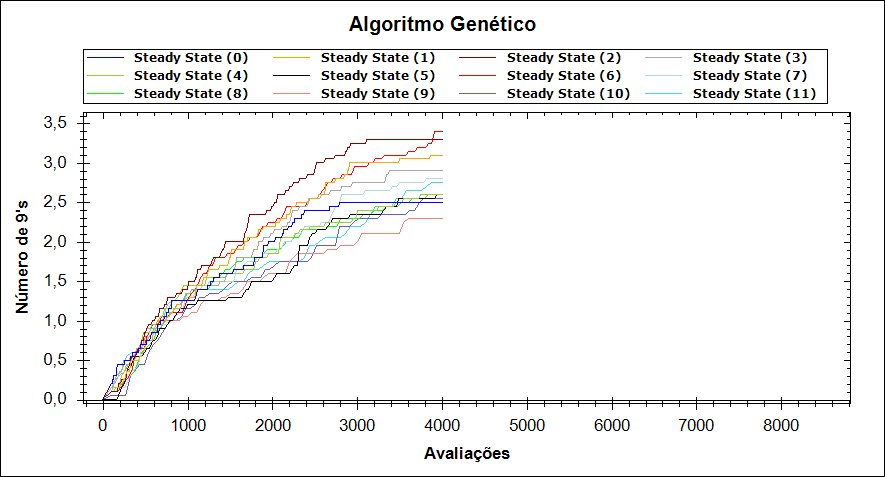
\includegraphics[scale = 0.65]{images/q2.png}
\caption{AG com Steady-State}
\end{figure}

\begin{figure}[H]
\centering
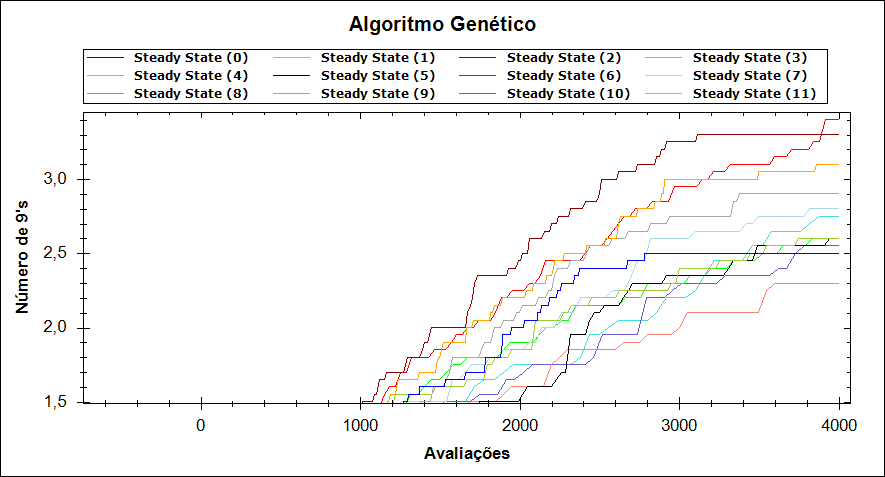
\includegraphics[scale = 0.65]{images/q2.2.png}
\caption{AG com Steady-State (zoom)}
\end{figure}

\subsection{Análise dos gráficos}
\textbf{Variedade de Curvas}: As curvas representam uma variedade de configurações de GAP, aumentando progressivamente. Essa extensão permite observar o comportamento do algoritmo sob um espectro mais amplo de perturbações genéticas.\\

\textbf{Performance Geral}: O gráfico mostra uma tendência geral onde, conforme o GAP aumenta, o desempenho inicial do algoritmo se mantém semelhante, mas as diferenças se tornam mais pronunciadas após aproximadamente 1000 avaliações.\\

\textbf{GAPs Menores (Steady State 0 a 5)}: Estas curvas tendem a se aglomerar mais na parte inferior do gráfico, sugerindo que substituições menores podem estar limitando a capacidade do algoritmo de explorar eficientemente o espaço de soluções, ou que o algoritmo pode estar demorando mais para convergir.\\

\textbf{GAPs Moderados (Steady State 6 a 9)}: Curvas neste intervalo mostram uma performance robusta, alcançando melhores níveis de fitness mais rapidamente que os GAPs menores. Isso indica um equilíbrio efetivo entre manter a diversidade genética e introduzir novas características.\\

\textbf{GAPs Maiores (Steady State 10 e 11)}: As curvas para GAPs maiores, como 10 e 11, começam a mostrar uma divergência em termos de performance. A curva para Steady State 10, em particular, mostra uma melhoria considerável em relação aos menores, mas a curva para Steady State 11 indica que um GAP ainda maior pode estar causando uma perda excessiva de informações genéticas úteis, resultando em uma performance piorada após certo ponto.\\

\subsection{Interpretação dos resultados}

Os GAPs que mostram uma melhoria grande e sustentada na aptidão ao longo das avaliações parecem ser aqueles na faixa moderada. Estes GAPs são grandes o suficiente para facilitar uma boa exploração do espaço de soluções, mas não tão grandes a ponto de degradar rapidamente a qualidade genética da população.\\

A tendência observada sugere que um GAP muito grande pode introduzir instabilidade na evolução do algoritmo, levando a um pico de performance seguido por uma estabilização ou mesmo declínio na qualidade das soluções encontradas.\\

Os GAPs moderados, provavelmente em torno de 20-30\% do tamanho da população, parecem oferecer o melhor desempenho. Eles equilibram a introdução de novas características genéticas com a manutenção de suficiente estabilidade genética para permitir que o algoritmo refine essas características em busca de soluções ótimas. Esta análise sugere que mais testes podem ser úteis para refinar ainda mais o valor ideal de GAP, especialmente para determinar o ponto exato onde um aumento adicional começa a ter retornos decrescentes ou mesmo negativos.



%%%%%%%%%%%%%%%%%%%%%%%%%%%%%%%%%%%%%%%
\newpage
\section{Taxas de Crossover e Mutação}
\textbf{Verificar o que acontece quando se roda o GA2-1 (20 vezes cada uma com 20 rodadas ou experimentos) com 
taxa de crossover muito baixa (pouca recombinação em torno de 10\%) e alta taxa de mutação (muitas mudanças 
aleatórias em torno de 80\%).} \\

\textbf{Comparar com o resultado do GA2-1 obtido no item 1.}\\

\begin{figure}[H]
\centering
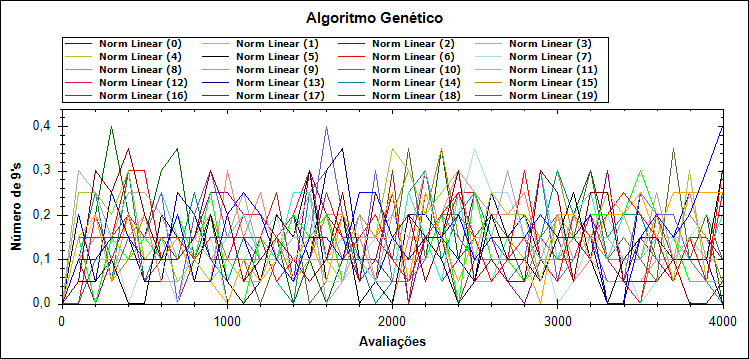
\includegraphics[scale = 0.65]{images/q3.png}
\caption{Tentativas para GA2-1 com 20 rodadas - Gráfico}
\end{figure}

\begin{figure}[H]
\centering
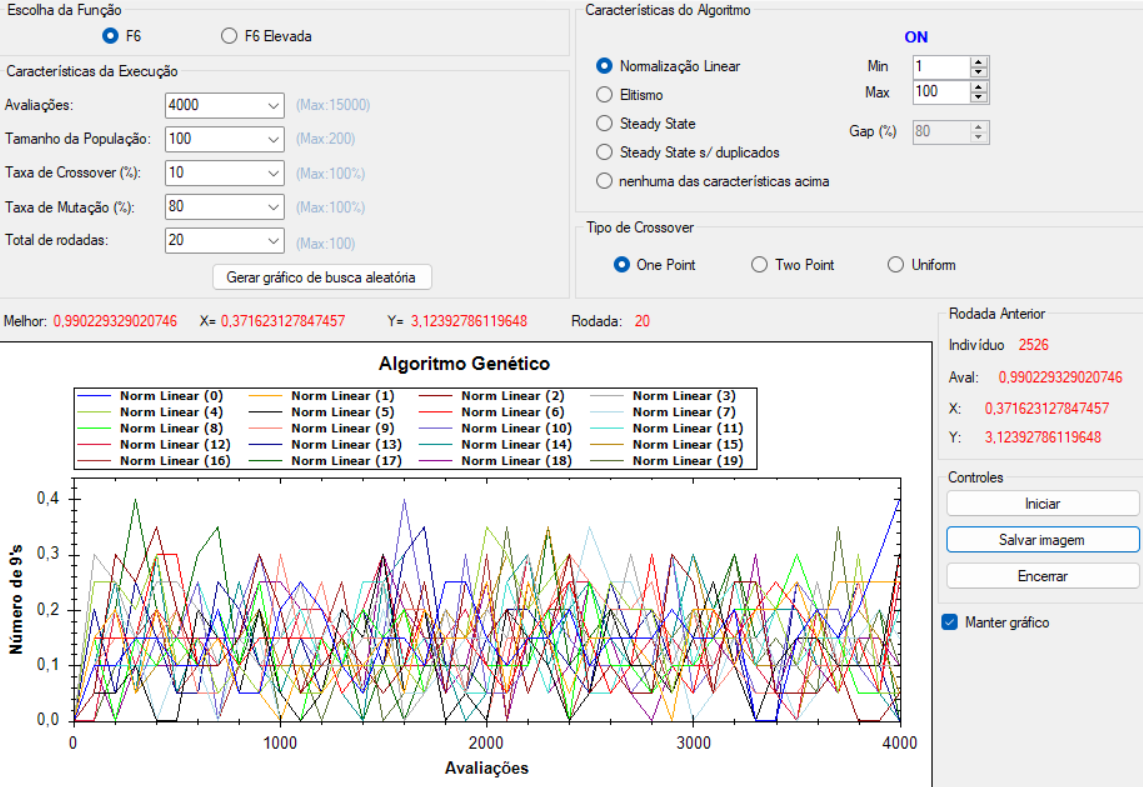
\includegraphics[scale = 0.65]{images/q3.2.png}
\caption{Tentativas para GA2-1 com 20 rodadas - GaDemo}
\end{figure}

Para esta etapa, realizamos os testes com taxa de crossover muito baixa 10\%) e uma alta taxa de mutação (80\%), como especificado na instrução.  

\subsection{Analisando a configuração do experimento}

\textbf{Configuração Original (GA2-1 do item 1):}

A curva laranja original representava um comportamento de crescimento estável com taxas de crossover e mutação padrão. Esta curva subiu de maneira gradual, indicando uma progressão eficiente e contínua na busca pela solução ótima.
Nova.\\

\textbf{Configuração com Baixo Crossover e Alta Mutação:}

A nova curva exibida mostra resultados consideravelmente diferentes. A variação nos resultados é muito maior, com picos significativos e muita flutuação. Essa configuração resultou em um comportamento muito menos previsível e potencialmente menos eficiente na convergência para soluções ótimas.

\subsection{Interpretação e Comentários}

Uma taxa de crossover baixa significa que há menos recombinação genética entre os indivíduos da população. Isso pode limitar a capacidade do algoritmo de combinar características benéficas de diferentes pais, o que normalmente ajuda a explorar eficientemente o espaço de solução.\\

Uma alta taxa de mutação introduz muitas alterações aleatórias nos indivíduos. Embora isso possa aumentar a diversidade genética e potencialmente ajudar a escapar de máximos locais, também pode perturbar combinações genéticas benéficas antes que elas possam ser totalmente exploradas. Além disso, mutações excessivas podem levar o algoritmo a uma exploração excessiva, afastando-se de áreas promissoras do espaço de 
busca.\\

Comparando com o resultado anterior do GA2-1 do item 1, a nova configuração parece menos eficaz em termos de progressão estável e convergência. A volatilidade do comportamento sugere que o equilíbrio entre exploração e explotação está inclinado demais para a exploração, o que não é ideal para a maioria dos problemas de otimização.\\

Então, parece que a alteração para uma baixa taxa de crossover e uma alta taxa de mutação não é benéfica para o desempenho do algoritmo genético no contexto deste problema específico. A configuração original, com taxas mais equilibradas, fornece uma abordagem mais controlada e eficiente, levando a uma melhoria consistente ao longo do tempo. Aqui fica bem ilustrado como mudanças extremas nos parâmetros podem afetar dramaticamente a eficácia de um algoritmo genético e destaca a importância de ajustar cuidadosamente essas taxas para balancear entre manter a diversidade genética e promover a convergência para soluções de alta qualidade.



%%%%%%%%%%%%%%%%%%%%%%%%%%%%%%%%%%%%%%%%%%%
\newpage
\section{Tamanho da População}
\textbf{Analisar o efeito do tamanho da população, obtendo as curvas de desempenho do GA2-2 (20 rodadas) para vários 
tamanhos de população (ex: 20, 50, 100, 150) e sempre com o mesmo número de gerações (total de indivíduos 
variável).}\\
%Imprimir as curvas tirar conclusões sobre o efeito do tamanho da população no desempenho do  algoritmo genético.

Para este item, então, iremos considerar um número fixo de 40 gerações para executar o GA2-2 dentro das especificações. Como manteremos 40 gerações para cada teste, deveremos variar os tamanhos da população e, portanto, multiplicar o tamanho da população pelo número de gerações para calcular o número total de avaliações individuais.\\

\subsection{Cálculo do Número Total de Avaliações
}

\subsubsection{20 populações}
\begin{equation*}
    Tamanho\_da\_População = 20
\end{equation*}
\begin{equation*}
    Número\_de\_Gerações = 40
\end{equation*}
\begin{equation*}
    Total\_de\_Avaliações = 20 \>\ (indivíduos) * 40 \>\ (gerações) = 800 \>\ avaliações
\end{equation*}

\subsubsection{50 populações}
\begin{equation*}
    Tamanho\_da\_População = 50
\end{equation*}
\begin{equation*}
    Número\_de\_Gerações = 40
\end{equation*}
\begin{equation*}
    Total\_de\_Avaliações = 50 \>\ (indivíduos) * 40 \>\ (gerações) = 2000 \>\ avaliações
\end{equation*}

\subsubsection{100 populações}
\begin{equation*}
    Tamanho\_da\_População = 100
\end{equation*}
\begin{equation*}
    Número\_de\_Gerações = 40
\end{equation*}
\begin{equation*}
    Total\_de\_Avaliações = 100 \>\ (indivíduos) * 40 \>\ (gerações) = 4000 \>\ avaliações
\end{equation*}

\subsubsection{150 populações}
\begin{equation*}
    Tamanho\_da\_População = 150
\end{equation*}
\begin{equation*}
    Número\_de\_Gerações = 40
\end{equation*}
\begin{equation*}
    Total\_de\_Avaliações = 150 \>\ (indivíduos) * 40 \>\ (gerações) = 6000 \>\ avaliações
\end{equation*}

\subsection{Resultados}
\begin{figure}[H]
\centering
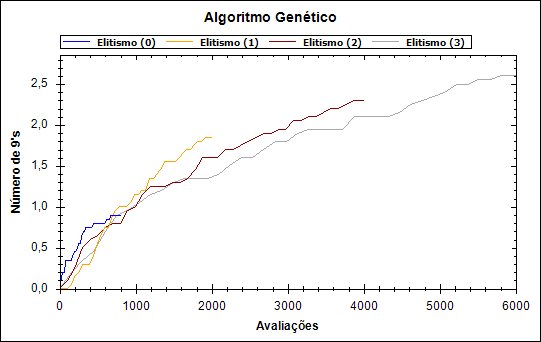
\includegraphics[scale = 0.85]{images/q4.png}
\caption{GA2-2: Tentativas para diferentes tamanhos de população}
\end{figure}

\textbf{Curva Azul (População de 20)}: Esta curva mostra o crescimento mais lento em termos de melhoria na aptidão ao longo das avaliações. A convergência é gradual e não atinge níveis tão altos de aptidão como as outras curvas. Isso pode indicar que uma população menor pode não explorar suficientemente o espaço de busca, limitando seu potencial para encontrar soluções ótimas.\\

\textbf{Curva Laranja (População de 50)}: A melhoria na aptidão é mais rápida e mais estável em comparação com a população de 20. Este tamanho de população parece oferecer um melhor equilíbrio entre exploração e explotação, permitindo que o algoritmo melhore de forma mais eficaz a aptidão ao longo do tempo.\\

\textbf{Curva Marrom (População de 100)}: Mostra um desempenho semelhante à curva laranja nos estágios iniciais, mas parece superá-la em termos de aptidão alcançada à medida que as avaliações progridem. Isso sugere que uma população ainda maior pode facilitar uma melhor exploração do espaço de busca, resultando em um desempenho aprimorado.\\

\textbf{Curva Cinza (População de 150)}: Esta curva demonstra o maior nível de aptidão ao final das avaliações. Apesar de ter uma trajetória similar à curva marrom durante as primeiras avaliações, ela se destaca nos estágios mais tardios, indicando que uma maior diversidade genética na população pode ser crucial para alcançar as melhores soluções.\\

Portanto, podemos concluir que populações maiores tendem a manter uma maior diversidade genética, o que ajuda a evitar mínimos locais e potencialmente descobrir soluções mais ótimas.\\

Populações maiores também permitem uma melhor exploração do espaço de busca, enquanto populações menores podem ser limitadas pela falta de diversidade genética, resultando em uma convergência prematura para soluções subótimas.\\

Embora populações maiores possam oferecer melhor desempenho, elas também requerem mais recursos computacionais e tempo para processamento. Portanto, encontrar o tamanho ótimo da população envolve balancear esses fatores com os benefícios de desempenho.


\newpage
\section{Convergência}
\textbf{Repetir o GA2-1 e o GA2-2 (20 rodadas cada) modificando apenas o total de indivíduos criados para o 10000. 
Imprimir as curvas em dois gráficos separados, um para o GA2-1 e outro para o GA2-2, e verificar se 
é vantajoso todo esse esforço computacional, em outras palavras, determinar o número de indivíduos para o qual cada algoritmo converge.}

\subsection{Resultado - GA2-1}

\begin{figure}[H]
\centering
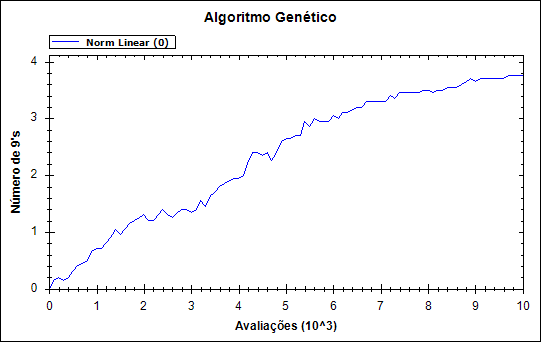
\includegraphics[scale = 0.85]{images/q5._GA21.png}
\caption{GA2-1 com 10000 indivíduos}
\end{figure}

A curva mostra um aumento constante na aptidão ao longo das avaliações. A tendência é progressiva, mas a curva suaviza à medida que se aproxima das 10 mil avaliações. Isso indica que, embora a normalização linear ajude a manter as avaliações dentro de uma escala consistente, o algoritmo ainda consegue fazer progressos ao explorar o espaço de busca.\\
A suavização da curva no final pode sugerir que o algoritmo está se aproximando de uma convergência, ou que está se tornando mais desafiador fazer melhorias significativas na aptidão à medida que se explora mais profundamente o espaço de soluções.

\subsection{Resultado - GA2-2 (Elitismo)}

\begin{figure}[H]
\centering
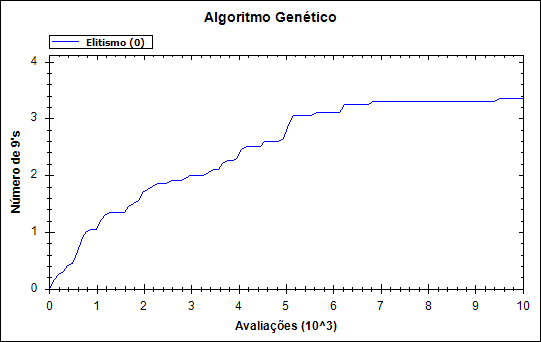
\includegraphics[scale = 0.85]{images/q5._GA22.png}
\caption{GA2-2 com 10000 indivíduos}
\end{figure}

Este gráfico mostra uma trajetória de desempenho um pouco mais escalonada comparada ao GA2-1. A aptidão melhora significativamente e, semelhante ao GA2-1, a curva começa a se estabilizar à medida que se aproxima das 10 mil avaliações. O platô final é mais pronunciado do que no GA2-1, indicando que o algoritmo pode ter alcançado uma convergência onde os indivíduos de elite dominam a população, limitando assim a introdução de novas características genéticas.\\
O impacto do elitismo é evidente, especialmente nas fases mais tardias do gráfico, onde o algoritmo mantém ou melhora ligeiramente a aptidão, mas com uma taxa de melhoria reduzida, sugerindo uma possível convergência prematura ou estabilização no espaço de busca.

\subsection{Conclusões}
Ambos os algoritmos mostram que aumentar o número de avaliações para 10.000 tem um impacto positivo na melhoria da aptidão, embora o benefício incremental pareça diminuir com o tempo. Isso é especialmente verdadeiro para o GA2-2 com elitismo, onde o platô sugere uma limitação na eficácia de continuar a aumentar as avaliações sem ajustes adicionais na estratégia genética.\\

O GA2-2 com elitismo parece convergir mais claramente para uma solução ótima, embora isso possa também limitar a diversidade genética. Por outro lado, o GA2-1 com normalização linear mostra uma melhoria mais gradual, sugerindo que pode continuar explorando novas áreas do espaço de busca mais eficazmente do que o GA2-2.\\

Ambas as estratégias têm seus méritos. O GA2-1 pode ser preferível para problemas que requerem uma exploração contínua do espaço de soluções, enquanto o GA2-2 pode ser mais adequado para cenários onde alcançar uma solução ótima rapidamente é mais crítico, mesmo que isso possa resultar em menor diversidade genética no final das execuções.\\

Essa análise ilustra que, enquanto aumentar o número de avaliações geralmente melhora o desempenho, o retorno diminui com o tempo e as estratégias adicionais podem ser necessárias para manter ou melhorar a eficácia do algoritmo em populações grandes.\\


\newpage
\section{Crossover}
\textbf{Comparar o efeito dos 3 tipos de crossover disponíveis na ferramenta, executando o GA2-1 (s/ elitismo) e o GA2-
2 (c/elitismo) com apenas 2500 indivíduos (20 rodadas) para cada tipo de crossover, usando taxa de crossover 
80\%.}
%Imprimir as curvas em dois um gráficos separados , um para o GA2-1 e outro para o GA2-2, e tirar  conclusões a respeito da característica conservadora/destrutiva de cada crossover.

\subsection{Resultado: GA2-1 (s/ elitismo)}
\begin{figure}[H]
\centering
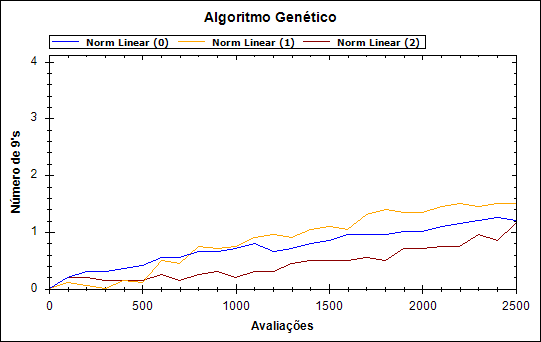
\includegraphics[scale = 0.85]{images/q6_GA21.png}
\caption{Diferentes tipos de crossover para GA2-1}
\end{figure}

\textbf{Crossover de 1 ponto (curva azul)}: O crossover de um ponto, embora conserve grandes blocos de genes, oferece uma melhoria contínua, mas não a mais agressiva. É eficaz, mas sua natureza conservadora pode limitar a exploração de novas combinações genéticas que poderiam levar a um salto na aptidão.\\

\textbf{Crossover de 2 pontos (curva laranja)}: O crossover de dois pontos permite uma introdução mais balanceada de diversidade genética, cortando e reorganizando os genes dos pais em dois pontos diferentes. Isso parece ser bastante efetivo, permitindo uma combinação mais diversa e potencialmente vantajosa de genes, o que se reflete em uma melhoria mais rápida e consistente na aptidão.\\

\textbf{Crossover uniforme (curva marrom)}:  Embora o crossover uniforme introduza uma alta diversidade genética ao misturar genes dos pais de maneira aleatória, neste contexto, ele não parece traduzir essa diversidade em uma melhoria rápida de aptidão. Isso pode sugerir que, embora explore novas combinações genéticas, essas combinações não estão necessariamente resultando em indivíduos mais aptos, possivelmente devido à criação de combinações subótimas ou ao desmantelamento de conjuntos de genes benéficos.\\

\subsection{Resultado: GA2-2 (c/ elitismo)}
\begin{figure}[H]
\centering
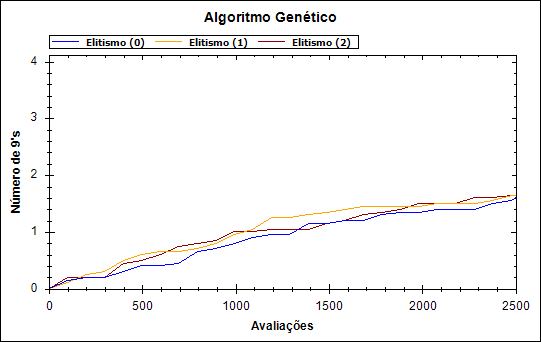
\includegraphics[scale = 0.85]{images/Q6_GA22.png}
\caption{Diferentes tipos de crossover para GA2-2}
\end{figure}

\textbf{Crossover de 1 ponto (curva azul)}: Apresenta uma melhora progressiva. Com o suporte do elitismo, parece que a preservação de blocos de genes se torna mais vantajosa, pois genes benéficos são mantidos.\\

\textbf{Crossover de 2 pontos (curva laranja)}: Similar ao crossover de 1 ponto, mas com uma ligeira vantagem em algumas áreas, possivelmente devido à capacidade de reorganizar eficazmente características valiosas de diferentes pais.\\

\textbf{Crossover uniforme (cura marrom)}: A curva mostra uma trajetória similar às outras, mas com um desempenho levemente superior no final, sugerindo que mesmo com elitismo, a introdução de diversidade genética por meio de um método aleatório pode ser benéfica.\\

\subsection{Conclusões}
No GA2-1, o crossover de dois pontos é o mais eficaz neste cenário, proporcionando uma combinação equilibrada de conservação e inovação, que efetivamente explora o espaço de busca genética e resulta em melhorias rápidas e significativas na aptidão.\\
O crossover de um ponto, embora estável, não oferece o crescimento mais rápido, mas ainda assim é capaz de proporcionar melhorias consistentes. Já o crossover uniforme parece ser menos eficaz do que o esperado para este conjunto de dados, indicando que a introdução aleatória de genes pode não ser sempre benéfica, especialmente se não for acompanhada por mecanismos que garantam a retenção de combinações de genes benéficas.\\

No GA2-2, todos os tipos de crossover parecem beneficiar-se do elitismo, com o uniforme mostrando uma ligeira vantagem ao final, indicando que a combinação de preservação de genes de elite com a introdução de novas combinações aleatórias pode ser ideal.\\

Estes resultados destacam a importância de escolher uma estratégia de crossover apropriada com base na presença ou ausência de elitismo e nas características específicas do problema a ser resolvido. A escolha adequada pode significativamente afetar a velocidade e a qualidade da convergência do algoritmo genético.



\newpage
\section{Normalização Linear}
\textbf{Repetir o GA2-3 COM GAP = 75 (considerando duplicados) e 50 rodadas para vários valores de máximo da 
normalização. Verificar o que acontece quando o valor de máximo aumenta e diminui (avaliar para os valores  10, 50, 100, 200, 300).}\\
%Imprimir as curvas em apenas um gráfico e tirar breves conclusões .

\subsection{Análise das curvas}

\begin{figure}[H]
\centering
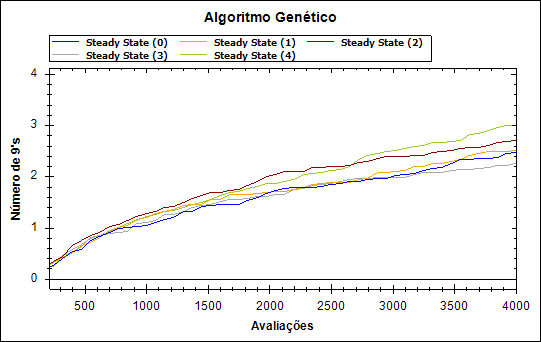
\includegraphics[scale = 0.85]{images/q7.png}
\caption{GA2-3 com diferentes máximos de normalização}
\end{figure}


\textbf{Curva marrom (max = 100)}: Apesar de um valor de normalização menor em comparação com 300, esta curva também mostra um bom desempenho, indicando que um valor de 100 pode ser suficiente para manter uma diversidade genética adequada e pressão seletiva para este caso específico, sem precisar de um escalonamento tão alto quanto 300.

\textbf{ Curva Verde (Max = 300)}: Esta curva, sendo a mais alta, sugere que uma normalização com um valor máximo de 300 está permitindo uma diferenciação mais eficaz entre os indivíduos de alta e baixa aptidão. Isso facilita uma seleção mais precisa e uma melhor exploração do espaço de busca, resultando em uma aptidão mais elevada.\\    

\textbf{Curvas azul (max = 10), laranja (max = 50) e cinza (max = 200)}: Estas curvas estão consistentemente mais baixas, especialmente a curva azul (Max = 10) e a laranja (Max = 50), o que indica que esses valores de normalização podem ser muito restritivos ou inadequados para diferenciar eficazmente as aptidões, limitando o desempenho geral.


\newpage
\section{Gerais}
\textbf{Fazendo variações nos parâmetros e técnicas disponíveis no GADEMO, estude livremente o efeito de cada um 
destes no desempenho de algoritmos genéticos. Destaque e explique uma importante constatação.}\\

Foram feitos alguns testes mantendo fixados o número de avaliações (10000), tamanho da população (100), taxa de crossover (65\%), taxa de mutação (0.8\%) e 20 rodadas. \\

Neste caso, foram executados testes com normalização linear, elitismo, steady-state com e sem duplocados para os 3 diferentes tipos de crossover. \\

Nas diferentes características variáveis, observamos que o crossover uniforme manteve um desempenho consistente, destacando-se em todas as configurações citadas acima.\\


O crossover uniforme trata cada gene de forma independente, escolhendo aleatoriamente de qual pai o gene será herdado. Isso promove uma diversidade genética significativa dentro da população, crucial para explorar efetivamente o espaço de busca e evitar convergências prematuras para mínimos locais.\\ 
Ao não se restringir a blocos fixos de genes (como no crossover de um ou dois pontos), o crossover uniforme pode combinar características benéficas de ambos os pais de maneira mais flexível e abrangente, potencialmente alcançando combinações de genes que são mais adaptados às exigências do ambiente de otimização.\\
Temos também uma robustez em diferentes configurações. A consistência do crossover uniforme em diferentes configurações do algoritmo, como normalização linear, presença ou ausência de elitismo e steady state com e sem duplicados, indica que sua eficácia não é fortemente dependente de características específicas do algoritmo. Isso o torna uma escolha versátil e confiável para uma variedade de problemas.\\

\textbf{Implicações práticas} \\

\begin{itemize}
    \item \textbf{Seleção de crossover}: Para problemas que exigem uma exploração intensiva do espaço de busca e onde a diversidadade genética é um fator crítico para o sucesso, o crossover uniforme pode ser a escolha preferencial.
    \item \textbf{Adaptação a mudanças}: O sucesso do crossover uniforme em manter a performance superior em diferentes configurações sugere que ele pode ser particularmente útil em ambientes dinâmicos ou em problemas onde os parâmetros podem mudar ao longo do tempo.
    \item \textbf{Desenvolvimento estratégico de otimização}:  Incorporar o crossover uniforme como parte de uma estratégia de otimização mais ampla, talvez em combinação com outras técnicas como mutação adaptativa e seleções focadas, pode melhorar ainda mais a eficácia dos algoritmos genéticos.
\end{itemize}

Portanto, o sucesso repetido do crossover uniforme utilizando as características de otimização, elitismo e steady state ressalta a importância de selecionar e configurar cuidadosamente os operadores genéticos com base nas características específicas de um dado problema. Além disso, destaca a necessidade de testes extensivos e análise comparativa para entender completamente como diferentes técnicas e parâmetros afetam o desempenho do algoritmo.\\

\textbf{Inibindo as características do algoritmo} \\

Por outro lado, ao optar por manter em "OFF" as características do algoritmo, alternando pelos diferentes tipos de crossover, identificamos que o crossover uniforme não performou tão bem quanto os outros dois tipos. Isso é interessante, pois destoa das observações feitas anteriormente.\\

A função $f_6$ possui uma paisagem de otimização complexa com muitos mínimos locais. A eficácia do tipo de crossover pode variar significativamente dependendo das características específicas do problema, como a topologia do espaço de busca.\\




























% REFERENCIAS %%%%%%%%%%%%%%%%%%%%%%%%%%%%%%%%%%%%%%%%%%%%%%%%%%%%%%%%%%%%%%



\end{document}